% Dokumentenklasse (festgelegt!)
\documentclass{llncs}

% Allgemeine Einstellungen
\usepackage[utf8]{inputenc} % Zeichenkodierung auf UTF8
\usepackage[ngerman]{babel} % Deutsche Anpassungen, z.B. Trennregeln
\usepackage[T1]{fontenc} % T1-Zeichenkodierung einschalten, damit z.B. Umlaute im PDF-Dokument gesucht werden können

%\usepackage[a4paper,top=3cm,bottom=2cm,left=3cm,right=3cm,marginparwidth=1.75cm]{geometry}

% Quellenverzeichnis:
\usepackage[backend=biber, style=numeric, sorting=none]{biblatex}
\addbibresource{Seminar_Quellenverzeichnis.bib}

% für TODO Kommentare:
\usepackage{todonotes}

% Quellcode-Abbildungen:
\usepackage{listings}

% Vektorgrafiken
\usepackage{svg}

% Tabellenbeschriftung
\usepackage{caption}
\captionsetup[table]{position=below,skip=1em}

% Farbe in Tabellenzellen:
\usepackage{colortbl}
\definecolor{hellgrau}{rgb}{0.95,0.95,0.95} % Farbdefinition, kann im Code verwendet werden

% Bilder einbinden:
\usepackage{graphics}
\graphicspath{{./img/}} % Angabe von Ordner für Bilder
\usepackage{subcaption}


\begin{document}
\title{Intertask Kommunikation in Echtzeitbetriebssystemen}
\author{Stefan Lindörfer\\
\email{stefan.lindoerfer@stud-mail.uni-wuerzburg.de}
}
\institute{
	Seminar: Embedded Systems\\bei Prof. Dr. Reiner Kolla\\Wintersemester 2020/21}

\date{\today}

\maketitle

\renewcommand{\abstractname}{Abstract}

\begin{abstract}
	Die Informationsübermittlung zwischen Tasks in Echtzeitbetriebssystemen ist von fundamentaler Bedeutung und kann je nach Anforderungsszenario auf verschiedene Arten erfolgen. In der vorliegenden Arbeit wird ein Überblick über die verschiedenen Möglichkeiten der Koordinierung und Synchronisierung von Tasks gegeben und anschließend vertieft gezeigt, wie Daten zwischen Tasks ausgetauscht werden können.
\end{abstract}

\section{Einführung}
\label{subsec:Einführung}
Echtzeitbetriebssysteme (auch \textbf{R}eal \textbf{T}ime \textbf{O}perating \textbf{S}ystems, kurz RTOS genannt) sind aus der Informatik nicht mehr wegzudenken und begegnen uns oft unbewusst im Alltag in zahlreich verschiedenen Anwendungsbereichen. So werden sie etwa in modernen Automobilen als Betriebssysteme eingesetzt, zur Steuerung und Regelung industrieller Anlagen verwendet oder im Verkehrswesen (z.B. Schienenverkehr- oder Ampelsteuerungen) genutzt \autocite[vgl.][157]{Winzker2008}. Auch als Betriebssysteme von Satelliten in der Raumfahrt sowie für den Einsatz in Luftfahrzeugen sind sie geeignet \autocite[vgl.][]{Systems2017} \autocite[vgl.][]{RODOS2017}.\\

Die Besonderheit dieser Art von Betriebssystemen ist die Fähigkeit, Echtzeit-Anforderungen umsetzen zu können. Das bedeutet (anders als bei Nicht-RTOS) als Softwareentwickler die Zusicherung seitens des Betriebssystems zu besitzen, dass eine bestimmte Aufgabe innerhalb eines vordefinierten Zeitfensters entweder ausgeführt und ggf. abgeschlossen (oder unterbrochen) wird. Betriebssysteme anderer Kategorien (z.B. Microsoft Windows) führen ihre Aufgaben meist schnellstmöglich bzw. ohne Vorhersagemöglichkeit aus und passen kein Zeitfenster ab, garantieren also keine Echtzeit, sondern setzen auf größtmögliche Performanz \autocite[vgl.][317]{HeinzWoern2005}.\\

Aufgaben in Echtzeitbetriebssystemen sind in sogenannte Tasks (oder auch Threads) unterteilt, die vom Betriebssystem getrennt voneinander verwaltet werden. Abhängig vom jeweiligen Szenario können Tasks jedoch nicht ausschließlich getrennt voneinander operieren und ihren jeweiligen Aufgaben nachgehen, sondern ein Informationsaustausch zwischen ihnen ist erforderlich: Um etwa einen Ablauf abzubilden, bei dem zuerst Task A und anschließend Task B ausgeführt werden soll, muss zunächst eine Information von A nach B übermittelt werden können, die den entsprechenden Prozessfortschritt anzeigt, sodass B beginnen kann. Aber auch wenn Daten eines Tasks von einem anderen zur (synchronisierten) Weiterverarbeitung benötigt werden, ist ein entsprechender Kommunikationskanal erforderlich um die Daten zu transferieren.\\

Dieser gesamte interne Informationsaustausch wird als Intertask-Kommunikation bezeichnet. Es existieren mehrere allgemeine Möglichkeiten und Techniken, Informationen und Daten zwischen Tasks auszutauschen, abhängig vom jeweiligen Szenario und den Anwendungsanforderungen. Diese Techniken werden im Folgenden aufgezeigt und nacheinander erläutert.

\subsection{Überblick}
\label{subsec:Überblick}
Grundsätzlich unterteilt man Intertask-Kommunikation in drei Kategorien \autocite[vgl.][79]{Cooling2017}:
\begin{enumerate}
	\setlength\itemsep{0.5em} % Zeilenabstand der Punkte ändern
	\item {Synchronisation und Koordination von Tasks ohne Datentransfer \label{subsec:Überblick:Punkt1}}
	\item {Datentransfer zwischen Tasks ohne Synchronisation \label{subsec:Überblick:Punkt2}}
	\item {Datentransfer zwischen Tasks mit Synchronisation \label{subsec:Überblick:Punkt3}}
\end{enumerate}
Punkt \ref{subsec:Überblick:Punkt1} enthält anders als \ref{subsec:Überblick:Punkt2} und \ref{subsec:Überblick:Punkt3} keinen Datentransfer und unterscheidet sich von diesen - wie bereits in der Einleitung ausgeführt - dadurch, dass lediglich eine Information ausgetauscht bzw. vom Empfänger abgefragt wird, um Tasks zu synchronisieren oder einen Arbeitsablauf umzusetzen. Während bei \ref{subsec:Überblick:Punkt2} und \ref{subsec:Überblick:Punkt3} ein Datentransfer insofern stattfindet, als das Daten ausgetauscht und vom Empfänger für die Weiterverarbeitung genutzt werden, sie also nicht zwingend für eine Ablaufsteuerung verwendet werden \autocite[vgl.][80]{Cooling2017}.

\subsection{Begriffsunterscheidung}
\label{subsec:Begriffsgrundlage}
Für eine genauere Betrachtung der einzelnen Kategorien aus Kapitel \ref{subsec:Überblick}, müssen zunächst die beiden Begriffe \textbf{Koordination} und \textbf{Synchronisation} definiert und pragmatisch voneinander abgegrenzt werden:
\begin{itemize}
	\setlength\itemsep{0.5em} % Zeilenabstand der Punkte ändern
	\item \textbf{Koordination}: \textit{\glqq Das Integrieren und Anpassen (einer Reihe von Teilen oder Prozessen), um eine reibungslose Beziehung zueinander herzustellen.\grqq{}} \autocite[80]{Cooling2017}
	\item \textbf{Synchronisation}: \textit{\glqq Etwas verursachen, bewegen oder ausführen, genau zur exakten Zeit.\grqq{}} \autocite[80]{Cooling2017}
\end{itemize}
Es fällt auf, dass die Definition der Koordination keinen Bezug zur Zeit beinhaltet. Der wesentliche Unterschied zwischen Koordinierung und Synchronisierung ist somit der Zeit-Faktor \autocite[vgl.][80]{Cooling2017}. Während mit einer Koordination ein theoretisch zeitunabhängiger, sequentieller Ablauf von Tasks angestrebt wird, meint Synchronisation dagegen das zeitliche Abgleichen von Vorgängen und legt damit verstärkt Fokus auf die Kerneigenschaft von Echtzeitbetriebssystemen. Dennoch haben beide Begriffe in dieser Thematik ihre klare Daseinsberechtigung und auch ihre bevorzugten Anwendungsgebiete in denen sie am besten zum Tragen kommen.

\section{Task-Interaktion ohne Datentransfer}
\label{sub:Task_Interaktion_ohne_Datentransfer}
Müssen, wie schon in Kapitel \ref{subsec:Überblick} erwähnt, keine Daten im eigentlichen Sinne zwischen Tasks transferiert werden, sondern nur ein Arbeitsablauf gesteuert werden, spricht man von Task-Interaktion ohne Datentransfer. Dies kann sowohl mit dem Ziel einer Synchronisation durchgeführt werden als auch zeit unkritisch als Koordination, siehe \ref{subsec:Begriffsgrundlage}. Demzufolge wird bei den Methoden dieser Kategorie auch in diese beiden Fälle unterschieden. Tabelle \ref{tab:Konstrukte} zeigt diese Unterscheidung auf und gibt gleichzeitig einen Überblick über die jeweils zu verwendeten Konstrukte.

\begin{table}
	\centering % Tabelle zentrieren
	\def\arraystretch{1.5} % Vertikales Padding
	\setlength{\tabcolsep}{0.5em} % Horizontales Padding
	\fbox{ % Rahmen um Tabelle
\begin{tabular}[h]{l|l|l}
	\textbf{Koordination} & \multicolumn{2}{c}{\textbf{Synchronisation}} \\
	\hline
	Condition Flags & Event Flags & Signale \\
	\hline
	\underline{\textit{Operationen:}} & \underline{\textit{Operationen:}} & \underline{\textit{Operationen:}} \\
	\texttt{Set} & \texttt{Set} & \texttt{Wait} \\
	\texttt{Clear} & \texttt{Clear} & \texttt{Send} \\
	\texttt{Check} & \texttt{Check} & \texttt{Check}
\end{tabular}}
	\caption{\label{tab:Konstrukte} Koordinierungs- und Synchronisationskonstrukte \autocite[vgl.][82]{Cooling2017}}
\end{table}
Grundsätzlich ist ein Flag (dt. Flagge) ein Statusindikator, der einen bestimmten Zustand anzeigt. Im simpelsten Fall sind das $0$ und $1$. Für das Ziel einer Koordinierung, werden sogenannte Condition Flags verwendet. Ist Synchronisierung erforderlich, dass also der gesteuerte Prozess zeitkritisch auszuführen ist, können - je nach Anwendungsfall - Event Flags oder Signale verwendet werden. Alle drei Konzepte werden im Folgenden detaillierter erläutert und Implementierungsansätze aufgezeigt.

\subsection{Task-Koordinierung mit Condition Flags}
\label{subsec:Koordinierung_mit_Condition_Flags}
Die einfachste Möglichkeit der Koordination ist das Condition Flag. Tabelle \ref{tab:Konstrukte} zeigt die auf Condition Flags anwendbaren Operationen \texttt{Set} (setzen), \texttt{Clear} (zurücksetzen) und \texttt{Check} (überprüfen).

\begin{figure}[h]
\centering
\def\svgwidth{300pt}
%\def\svgwidth{\columnwidth} % Breite wird auf Blattbreite (spalte) gesetzt
\input{ConditionFlag.pdf_tex}
\caption{\label{fig:ConditionFlag} Einfache Benutzung von Condition Flags \autocite[vgl.][83]{Cooling2017}}
\end{figure}

Abbildung \ref{fig:ConditionFlag} zeigt exemplarisch, wie Condition Flags verwendet werden: Task A übernimmt in diesem Fall die Steuerung des Ablaufs, während Task B darauf wartet ausgeführt zu werden und fortlaufend in regelmäßigen Abständen überprüft (\texttt{Check}), ob das zugehörige Flag gesetzt wurde. Im einfachsten Fall wird dafür eine globale Boolean-Variable eingesetzt, bei dieser $true$ den Zustand \glq gesetzt\grq{} und $false$ den Zustand \glq zurückgesetzt\grq{} repräsentieren kann. Ist es erforderlich, mehrere Zustände einzusetzen, können Aufzählungstypen wie Enums verwendet werden. Diese bieten auch den Vorteil der besseren Lesbarkeit des Quellcodes, da sofort verifizierbar ist, welcher Flag-Zustand \glq gesetzt\grq{} bzw. \glq zurückgesetzt\grq{} darstellt. Für die meisten Anforderungen ist dieses Vorgehen der Implementierung von Condition Flags absolut ausreichend \autocite[vgl.][84]{Cooling2017}.\\

In kritischeren Situationen jedoch, z.B. bedingt durch hohe Zugriffsraten auf ein Flag (es können sich Lese- oder Schreibfehler ergeben) oder wenn ein höheres Maß an Ausfallsicherheit (keine Redundanz) gewünscht ist, empfiehlt sich eine Mehrfachabsicherung wie sie Abbildung \ref{fig:ConditionFlag2} demonstriert:

\begin{figure} [h]
	\centering
	\def\svgwidth{300pt}
	%\def\svgwidth{\columnwidth} % Breite wird auf Blattbreite (spalte) gesetzt
	\input{ConditionFlagII.pdf_tex}
	\caption{\label{fig:ConditionFlag2} Verbesserte Benutzung von Condition Flags zur Koordination \autocite[vgl.][84]{Cooling2017}}
\end{figure}

Für jeden Zustand, der gesetzt werden kann (hier: zwei), existiert jetzt ein eigenes Condition Flag. Task A übernimmt in diesem Fall ausschließlich das Setzen der Zustände, führt diese Operation jedoch nur durch, falls das entsprechende Flag vorher von Task B zurückgesetzt wurde \autocite[vgl.][85]{Cooling2017}. Task B prüft im Unterschied zur Abbildung \ref{fig:ConditionFlag} jetzt zusätzlich den Zustand aller relevanten Flags (bezogen auf Abbildung \ref{fig:ConditionFlag2} also beide) bevor auf einen \texttt{Set}-Zustand reagiert wird \autocite[vgl.][85]{Cooling2017}. Wenn Unstimmigkeiten auftreten, weil z.B. das Prüfergebnis keinen eindeutig definierten Gesamtzustand ausweist, kann ein Fehlverhalten rechtzeitig abgefangen werden. Anders als dies bei Abbildung \ref{fig:ConditionFlag} möglich ist, denn dort kann u.U. kein Fehlverhalten vom Empfänger-Task festgestellt werden, da keine Absicherungsinstanz existiert, mit der verglichen werden könnte. Nach einem erfolgreichem \texttt{Check} wird das ausgeführte Flag wieder von Task B zurückgesetzt. Umgesetzt wird diese Methode wieder mittels Enums, wie folgender Codeabschnitt für Abbildung \ref{fig:ConditionFlag2} zeigen soll:
\begin{lstlisting}[language=C]
typedef enum {StartSet, StartClear} StartFlag;
typedef enum {StopSet, StopClear} StopFlag;
\end{lstlisting}
Diese Herangehensweise führt, wie bereits hervorgehoben, zu einer sichereren und zuverlässigeren Abwicklung der Koordination und besitzt auch die bereits festgestellte Eigenschaft der besseren Lesbarkeit, was nicht zu unterschätzen ist. An dieser Stelle sei noch erwähnt, dass eine Implementierung auf globaler Ebene ebenfalls Nachteile mit sich bringen kann (schlechtere Performanz, unkontrollierter Zugriff). In objektorientierten Programmiersprachen sollte deswegen eine Kapselung in einem separatem Objekt in Erwägung gezogen werden.\\

Eine weitere Möglichkeit der Organisation mit Condition Flags sind \textbf{Flag Gruppen}. Diese bieten sich besonders dann an, wenn viele Zustände abgebildet werden sollen, die zudem logisch miteinander in Verbindung stehen können. Wenn beispielsweise etwa in einem einfachen Fall Zustand A (Flag A) nicht gleichzeitig mit Zustand B (Flag B) gesetzt sein darf. Dabei werden einzelne Flags auf Wortbreite zusammengefasst \autocite[vgl.][85]{Cooling2017} (auch eine geringere Breite ist möglich, z.B. durch Einsatz einer Variablen geringerer Breite), in der jedes Bit ein Flag repräsentieren kann. Abbildung \ref{tab:FlagGroup} zeigt dieses Konzept auf einer 2 Byte Variablen mit je 8 Bits.\\
\begin{table}[h]
	\centering % Tabelle zentrieren
	\def\arraystretch{1.5} % Vertikales Padding
	\setlength{\tabcolsep}{0.5em} % Horizontales Padding
	%\fbox{ % Rahmen um Tabelle
		\begin{tabular}[h]{|l|c|c|c|c|c|c|c|c|c|c|c|c|c|c|c|c|}
			\hline
			\textbf{Bit} & \cellcolor{hellgrau}15 & \cellcolor{hellgrau}14 & \cellcolor{hellgrau}13 & \cellcolor{hellgrau}12 & \cellcolor{hellgrau}11 & \cellcolor{hellgrau}10 & \cellcolor{hellgrau}9 & \cellcolor{hellgrau}8 & \cellcolor{hellgrau}7 & \cellcolor{hellgrau}6 & \cellcolor{hellgrau}5 & \cellcolor{hellgrau}4 & \cellcolor{hellgrau}3 & \cellcolor{hellgrau}2 & \cellcolor{hellgrau}1 & \cellcolor{hellgrau}0 \\
			\hline
			\textbf{Wert} & 1 & 0 & 0 & 1 & 0 & 1 & 1 & 1 & 1 & 0 & 0 & 1 & 0 & 1 & 1 & 0 \\
			\hline
	\end{tabular}%}
	\caption{\label{tab:FlagGroup} Condition Flag Gruppe}
\end{table}

Wird der Wert der Variablen gelesen und als Integer (Ganzzahl) interpretiert (Abbildung \ref{tab:FlagGroup} - Wert: $38806$), kann er zudem bequem und einfach angepasst werden. Um etwa mehrere Flags, also Einzelbits, gleichzeitig zu setzen oder rückzusetzen, kann Bitmanipulation verwendet werden. Auch die Anwendung logischer Operatoren ($AND$, $OR$, $XOR$, $NOT$, $XNOR$) ist auf die einzelnen Bits möglich. Mit solchen Flag Gruppen kann daher beispielsweise leicht die logische Aussage
\begin{equation}
((([b_{15}] \wedge ([b_{13}] \vee \neg[b_{11}]))\oplus [b_{5}])\equiv 1)
\label{eq:ConditionFlagGroupEq}
\end{equation}
implementiert und evaluiert werden. Indem eine Bitmaske, die die relevanten Bits (hier: 15, 13, 11 und 5) markiert, mit dem $AND$-Operator auf den Variableninhalt aus Tabelle \ref{tab:FlagGroup} angewendet wird, erhält man eine gefilterte Bitfolge:
% Formatiert das lstlisting in die Mitte:
{
\lstset{basicstyle=\footnotesize, frame=tb, xleftmargin=.3\textwidth, xrightmargin=.29\textwidth}
\begin{lstlisting}[language=C]
  1001011110010110 (38806)
& 1010100000100000 (43040)
------------------
  1000000000000000 (32768)
\end{lstlisting}
}
Das Ergebnis enthält für unmarkierte Bits stets eine $0$ und für markierte eine $1$, sofern das jeweilige Bit der Variablen gesetzt war, ansonsten ebenfalls eine $0$. Dieses Resultat kann damit komfortabel für weitere Vergleiche herangezogen werden. Beispielsweise erfüllt $32768$ bereits die oben angegebene Gleichung (\ref{eq:ConditionFlagGroupEq}). Ein vollwertiger C++-Code für sogenanntes Bit Pattern, eine noch effizientere Möglichkeit der Analyse, ist unter \autocite{Turner2020} zu finden. Mit dieser Methode entfällt quasi der Filterungsprozess und der Variableninhalt kann sozusagen bereits vollständig in die Gleichung eingesetzt werden, während bei ersterer Methode, das Ergebnis nach dem Filtern noch untersucht werden muss. Für weitere ausführlichere Informationen zu diesem Thema sei auf die entsprechende Fachliteratur verwiesen.\\

Zusammengefasst sind Condition-Flags ein gutes Konstrukt um einen Ablauf von Tasks zu koordinieren. Es bieten sich für verschiedenste Anforderungen einfache und trotzdem leistungsstarke Lösungen an, um eine Koordinierung zu realisieren und die zugehörige Kommunikation sicher und zuverlässig zu gestalten.

\subsection{Einseitige Task-Synchronisation über Event Flags}
\label{subsec:Task-Synchronisation_Event_Flags}
Event Flags übernehmen viele Eigenschaften von Condition Flags wie sie in Kapitel \ref{subsec:Koordinierung_mit_Condition_Flags} vorgestellt wurden. Auf sie sind, wie in Tabelle \ref{tab:Konstrukte} dargestellt, auch die gleichen Operationen anwendbar: \texttt{Set} (setzen), \texttt{Clear} (zurücksetzen) und \texttt{Check} (überprüfen). Event Flags können anders als Condition Flags trotzdem zur Task-Synchronisation eingesetzt werden. Allerdings ist die erreichte Synchronisierung - wie noch gezeigt wird - auf eine Richtung beschränkt \autocite[vgl.][87]{Cooling2017}. Die im Vergleich zu Condition Flags neu hinzukommende Komponente ist das Ereignis (Event).\\

Ereignisse können asynchron und unvorhersehbar auftreten und - je nach Szenario - muss entsprechend schnell auf sie reagiert werden können, das entsprechende koordinierte Verhalten also möglichst synchron zum Zeitpunkt des Events ausgelöst werden \autocite{MikrocontrollerInterrupt}. Um dies zu erreichen, wird eine \textbf{I}nterrupt \textbf{S}ervice \textbf{R}outine (ISR) eingesetzt, die auf das Eintreten eines Events wartet und - so lange keines eingetreten ist - sich in einem suspendierten Zustand befindet \autocite[vgl.][87]{Cooling2017}. Ein Beispiel für ein solches Ereignis kann ein Hardware-Interrupt sein wie er in Abbildung \ref{fig:EventFlagBeispiel} gezeigt wird: Erst mit gedrücktem bzw. gehaltenem blauen Button leuchten die vier LEDs auf (siehe Abb. \ref{fig:EventFlagAn}).\\

\begin{figure}
	\centering
	\begin{subfigure}{.250\textwidth}
		%		\centering
		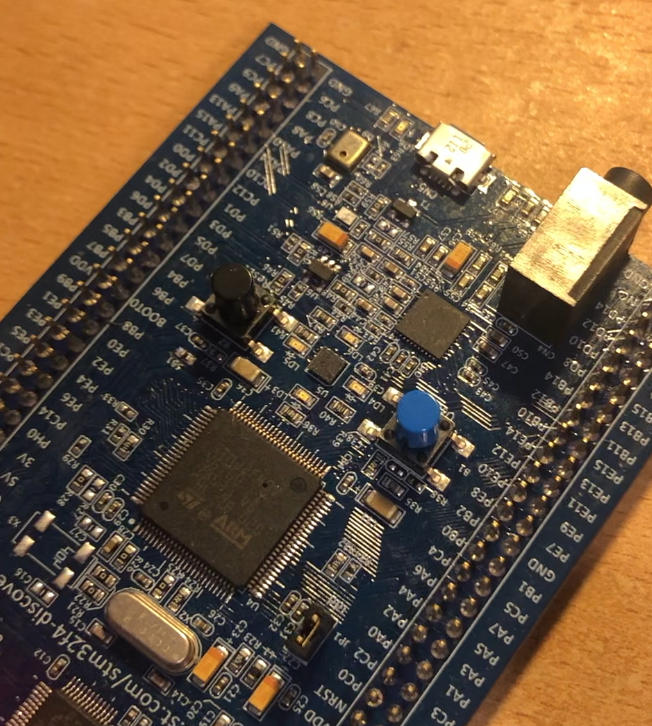
\includegraphics[width=\linewidth]{EventFlagsAus.jpg}
		\caption{suspendierte ISR}
		\label{fig:EventFlagAus}
	\end{subfigure}
	\hspace{1em}
	\begin{subfigure}{.250\textwidth}
		%		\centering
		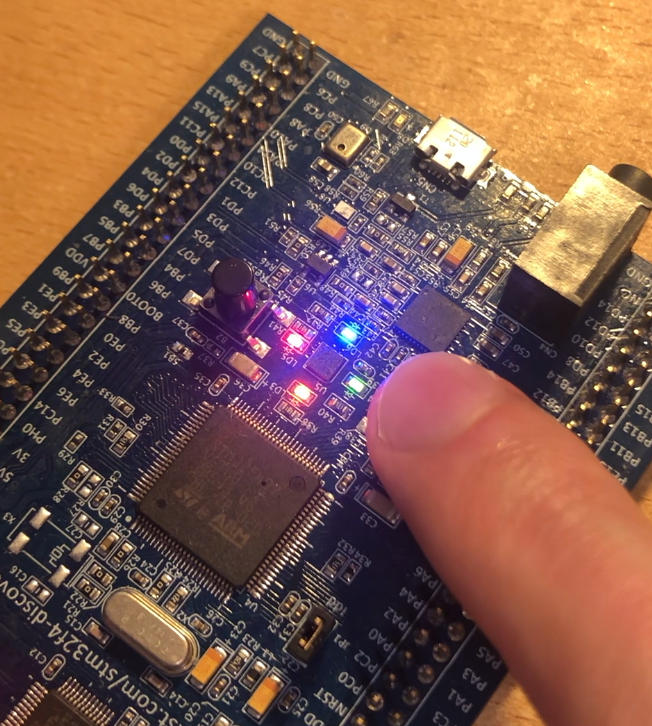
\includegraphics[width=\linewidth]{EventFlagsAn.jpg}
		\caption{aktive ISR}
		\label{fig:EventFlagAn}
	\end{subfigure}
	\caption{Beispiel von Event Flags für Interrupt-Management auf STM32F4 Discovery-Board}
	\label{fig:EventFlagBeispiel}
\end{figure}

Der schematische Ablauf mit Event Flags ist mit Abbildung \ref{fig:ConditionFlag} durchaus vergleichbar, nur dass Task A durch eine ISR ersetzt wird und eine Eingabe in Form des ausgelösten Ereignisses bekommt bevor das Event Flag gesetzt (oder rückgesetzt) wird \autocite[vgl.][87]{Cooling2017}. Als weiterführende Lektüre zum Thema Interrupt und Interrupt Service Routine wird \autocite{MikrocontrollerInterrupt} oder weitere Fachliteratur empfohlen. Dabei muss es sich nicht zwingend um ein Hardware-Interrupt handeln, auch auf andere, benutzerdefinierte Ereignisse kann so reagiert werden.

Weiterhin spielt für die hier gewünschten Task-Synchronisierung, also der Zeitraum, in dem der Empfänger Task B das Event Flag überprüft (\texttt{Check}), eine größere und wichtigere Rolle: Für eine dynamische Reaktion auf das Ereignis ist ein entsprechend kleines, periodisches Zeitfenster erforderlich. In Abbildung \ref{fig:EventFlagBeispiel} dargestellter Demonstration prüft Task B beispielsweise alle 500 Millisekunden ob das zugehörige Event Flag gesetzt ist. Ein darüber hinaus durchgefühter Versuch mit einer zwei-Sekunden-Periode funktionierte prinzipiell ebenfalls, zeigte aber kein flüssiges Verhalten von Aktion und Reaktion und kann deswegen für dieses Szenario ungeeignet sein. Hier muss von Anwendungsfall zu Anwendungsfall seperat entschieden werden.

Um das Betriebsystem zu entlasten, wird Task B nach jeder negativen Überprüfung bis zur nächsten Periode suspendiert, womit Ressourcen für andere Aufgaben frei werden.\\ 

Die Anwendung der unter Kapitel \ref{subsec:Koordinierung_mit_Condition_Flags} vorgestellten Techniken zu Condition Flags (z.B. Flag Gruppen) sind auch auf das Konstrukt der Event Flags übertragbar \autocite[vgl.][87-88]{Cooling2017}. Somit ist sowohl eine zuverlässigere und sicherere Implementierung wie auch für eine größere und ggf. auch verknüpftere Anzahl Event Flags vorhanden.\\

Wie eingangs bereits erwähnt, funktioniert diese Synchronisierung lediglich in eine Richtung: Die Interrupt Service Routine wird durch das vordefinierte Event geweckt und setzt das entsprechende Flag, welches vom Empfänger-Task im Rahmen seiner regelmäßigen Überprüfung registriert wird. Ist die Überprüfungsperiode entsprechend den Anforderungen gewählt, wird eine Synchronisierung von Ereignis und Reaktion bzw. ISR und Task B erreicht. Sollen zwei oder mehrere Tasks synchronisiert werden, bei der jeder beteiligte Task sowohl Sender als auch Empfänger sein kann, ist eine andere Methodik zu wählen. Diese wird im nächsten Abschnitt vorgestellt.

\subsection{Beiderseitige Task-Synchronisation über Signale}
\label{subsec:Task_Synchronisation_Signale}
Mit der bisher vorgestellten Technik, der Event Flags, lässt sich bereits eine einseitige Synchronisation implementieren. Bei einer Problemstellung aber, bei der zwei oder mehrere Tasks nach und nach in eine Art Wartestellung gehen (etwa weil ihre Aufgaben erfüllt sind) und alle zu einem gleichen (synchronen) Zeitpunkt erneut starten sollen, hilft dieses Konstrukt allerdings nicht weiter. Dafür gibt es das Konzept der Signale.\\

Die in Tabelle \ref{tab:Konstrukte} angegebenen Operationen \texttt{Wait} (warten), \texttt{Send} (senden) und \texttt{Check} (überprüfen) lassen bereits einen anderen Umgang als bei den bisher vorgestellten Flags aus Kapitel \ref{sub:Task_Interaktion_ohne_Datentransfer} erahnen: Eine zentrale Stelle (diese kann etwa das Betriebssystem bereitstellen) übernimmt die Signalverwaltung. Bei ihr registrieren sich die beteiligten Tasks sobald eine der o.g. Operationen ausgeführt wird (vgl. Abb. \ref{fig:Signale_gesamt}) und diese übernimmt auch die Steuerung dieses Konstrukts. Damit ist das Signal keinem spezifischem Task zugeordnet und auch keine direkt von diesem ausgehende Synchronisation \autocite[vgl.][91]{Cooling2017}. Genau dieser Umstand ermöglicht eine beiderseitige/mehrseitige Synchronisierung. Abbildung \ref{fig:Signale_gesamt} stellt die drei auftretenden Möglichkeiten vor.

\begin{figure}[h]
	\centering
	\fbox{
	\begin{subfigure}[t]{.353\columnwidth} % Werte mal so eingestellt lassen! .353
		\def\svgwidth{\columnwidth} % Breite wird auf Blattbreite (spalte) gesetzt
		\input{Signale_a.pdf_tex}
		\caption{\label{subfig:Signale_a}}
	\end{subfigure}
}\fbox{
	\begin{subfigure}[t]{.35\columnwidth} % Werte mal so eingestellt lassen! .35
		\def\svgwidth{\columnwidth}
		\input{Signale_b.pdf_tex}
		\caption{\label{subfig:Signale_b}}
	\end{subfigure}
}\fbox{
	\begin{subfigure}[t]{.1735\columnwidth} % Werte mal so eingestellt lassen! .1735
		\def\svgwidth{\columnwidth}
		\input{Signale_c.pdf_tex}
		\caption{\label{subfig:Signale_c}}
	\end{subfigure}
}
	\begin{subfigure}{.40\columnwidth} % Werte mal so eingestellt lassen! .40
		\def\svgwidth{\columnwidth}
		\input{Signale_Legende.pdf_tex}
	\end{subfigure}
	\caption{\label{fig:Signale_gesamt}Task-Synchronisation mittels Signalen \autocite[vgl.][90]{Cooling2017}}
\end{figure}

Zunächst sollen in den Abbildungen \ref{subfig:Signale_a} und \ref{subfig:Signale_b} zwei Tasks synchronisiert werden. Beide Darstellungen unterscheiden sich lediglich in der Reihenfolge, welche Operation zuerst auf ein Signal gewirkt wird: Der Task, welcher sich zuerst mit einer Operation meldet, wird suspendiert bis er - zusammen mit dem anderen Task - das Signal zur Wiederaufnahme erhält. Beide starten dann synchron zum gleichen Zeitpunkt \autocite[vgl.][90-91]{Cooling2017}.
Der sichtbare zeitliche Abstand bevor beide Tasks erneut starten, nachdem sie zur Synchronisierung gemeldet sind, kann darin begründet sein, dass zuerst ein Zeitfenster abgewartet werden soll oder ein Jitter (unvorhersehbare Verzögerung) auftritt, der den Start verzögert.

Abbildung \ref{subfig:Signale_c} zeigt, wie ein einzelner Task synchronisiert wird, ohne bekanntes Mitspiel anderer Tasks: Eine Überprüfung des Signalstatus erfolgt und ggf. eine Suspendierung oder eine sofortige Wiederaufnahme. Hierbei kann die Signalverwaltung (Exekutive) auch eine interne Logik besitzen und zum Timing verschiedener einzelner oder mehrerer Tasks benutzt werden \autocite[vgl.][91]{Cooling2017}.\\

Die Umsetzung von Signalen erfolgt normalerweise über Funktionen \autocite[vgl.][91]{Cooling2017}, wie im folgenden mit der Programmiersprache C skizziert:
\begin{lstlisting}[language=C]
/* Sendestatus auf das Signal */
void Send(SyncSignal SignalName);

/* Warte-Anfrage an Signal */
void Wait(SyncSignal SignalName);

/* Prueft ob ein Task wartet */
typedef enum {false, true} bool; // Def. fuer C hilfreich
bool Check(SyncSignal SignalName);
\end{lstlisting}
Zusammengefasst ist dabei folgendes, aus Abbildung \ref{fig:Signale_gesamt} abgeleitetes Verhalten in den Funktionen zu implementieren um Signale vollständig umzusetzen:
\begin{itemize}
	\item \texttt{Send}: Ausführender Task wird suspendiert, sofern kein anderer Task bereits eine \texttt{Wait}-Anfrage gestellt hat.
	\item \texttt{Wait}: Wird das Signal nicht bereits gesendet, wenn diese Anfrage gestellt wird, wird betreffender Task ebenfalls suspendiert. Andererseits wird der \glqq sendende \grqq{} Task reaktiviert und beide Tasks werden synchron wieder ausgeführt.
	\item \texttt{Check}: Gibt $true$ zurück, wenn das Signal gesendet wird, ansonsten $false$.
\end{itemize}
Somit sind Signale eine Möglichkeit, um in zwei oder mehrere Richtungen zu synchronisieren, da hier jeder Task sowohl Sender als auch Empfänger des Synchronisationsprozesses sein kann \autocite[vgl.][91]{Cooling2017}. Diese Technik wird allerdings von eher wenigen Echtzeitbetriebssystemen als Möglichkeit zur Synchronisierung angeboten \autocite[vgl.][91]{Cooling2017}.

\section{Datentransfer ohne Synchronisation oder Koordination}
\label{sub:Datentransfer_ohne_Sync_Koord}
Ist ein regelmäßiger Datenaustausch zwischen Tasks erforderlich (z.B. weil Daten zur Weiterverarbeitung benötigt werden), die aber nicht zur Koordination verwendet und ebenfalls nicht an zeitliche Kriterien gebunden sind, wird dies über verschiedene Datenverarbeitungsmechanismen bewerkstelligt. Diese lassen sich primär in zwei Kategorien unterteilen. Wie noch gezeigt wird, basieren sie auf allgemein bekannten Datenstrukturen.
\begin{figure}
	\centering
	\begin{subfigure}[b]{.450\textwidth}
		\def\svgwidth{\columnwidth}
		\input{RandomAccess.pdf_tex}
		\caption{\label{subfig:zufaelliger_Zugriff}Direkter Zugriff}
	\end{subfigure}
	\hspace{3em}
	\begin{subfigure}[b]{.450\textwidth}
		\def\svgwidth{\columnwidth}
		\input{SequentialAccess.pdf_tex}
		\caption{\label{subfig:sequentiell_Zugriff}Sequentieller Zugriff}
	\end{subfigure}
	\caption{\label{fig:Datentransfer_Ueberblick}Datentransfer zwischen Tasks \autocite[vgl.][95]{Cooling2017}}
\end{figure}

Abbildung \ref{fig:Datentransfer_Ueberblick} zeigt die Unterscheidung der hier aufgeführten zwei Prinzipien \glqq direkter Zugriff\grqq{}  (\ref{subfig:zufaelliger_Zugriff}) und \glqq sequentieller Zugriff\grqq{} (\ref{subfig:sequentiell_Zugriff}). Während bei ersterem eine Vielzahl an Tasks die gleiche Datenstruktur verwenden können, erfolgt bei zweiterem eine Eins-zu-Eins-Weiterleitung. Damit besitzt jeder Datentyp auch seine Daseinsberechtigung und wird im folgenden genauer vorgestellt.
\subsection{Pools}
\label{subsec:Pools}
Pools sind per Definition ein \glqq Read-Write Random Access Data Store\grqq{} \autocite[94]{Cooling2017}. Das bedeutet: Pools bieten einen direkten Zugriff, erlauben also den Zugang auf alle darin befindlichen Elemente. Außerdem besitzen sie eine variable Größe, ist also theoretisch nicht auf eine bestimmte, feste Anzahl an möglichen beinhalteten Elementen beschränkt. Er kann aber nur vordefinierte Objekte vom gleichen Typ speichern. Folgende Codedarstellung soll dieses Prinzip in C++ verdeutlichen:
\begin{lstlisting}[language=C++]
struct Data {
	char* id;
	int value;
};

Pool<Data> fifoList;
\end{lstlisting}
Ein Typ $Data$ wird deklariert, welcher einen $char$-Zeiger sowie einen Integer (Ganzzahl) enthält. $fifoList$ kann nach der Deklarierung nur Objekte dieses Typs aufnehmen und verwalten. Wie noch ausgeführt wird, bieten Pools allerdings - abhängig von der Implementierung - den Vorteil, dass sie nicht in einem zusammenhängenden Speicherblock untergebracht sein müssen. Hier sei der Vollständigkeit halber noch angemerkt, dass das Objekt, welches vom $char$-Zeiger referenziert wird, nicht im Speicherbereich des Pools liegt. Dessen Speicheradresse und der Integer allerdings schon.

Eine weitere Eigenschaft eines Pools ist damit die (Daten-)Kapselung: Außerhalb existierender Code bzw. Tasks erhalten lediglich Zugriff auf die Lese- und Schreib-Methoden des Pools, haben aber keinerlei Einfluss auf die interne Organisation der Daten oder Informationen über den Speicherort dieser.\\

\begin{figure}%{.250\textwidth}
	\centering
	\def\svgwidth{.50\columnwidth}

	\input{Pool.pdf_tex}
	\caption{\label{fig:Pool}Ein mit Mutex geschützter Pool \autocite[vgl.][95]{Cooling2017}}
\end{figure}

Diese Kapselung soll in Abbildung \ref{fig:Pool} dargestellt werden, sie zeigt außerdem den schematischen Aufbau dieses Datentyps: Über eine Schnittstelle (Interface), die mindestens die o.g. (Lese-/Schreib-)Methoden bereitstellt, erfolgt die Kommunikation bzw. die Datenübermittlung in beide Richtungen. Um Schreib- oder Lesefehler zu vermeiden, können Pools intern einen sogenannten Mutex, also einen Sicherungsmechanismus verwenden, der keinen mehrfach Zugriff auf Daten erlaubt. Abbildung \ref{fig:Pool} zeigt dessen Position und Funktionsweise: Tasks die während eines gerade stattfindenden Zugriffs ebenfalls Daten erlangen möchten, werden suspendiert und erhalten nach der internen Freigabe durch den Mutex nacheinander anschließend Zugriff auf die Daten. Dies ist vergleichbar mit einer Schrankenabfertigung im Straßenverkehr \autocite[vgl.][95]{Cooling2017}.\\

Allgemein bekannte Datenstrukturen die sich Pools zuzuordnen lassen, sind etwa FIFO (\textbf{F}irst \textbf{I}n \textbf{F}irst \textbf{O}ut) und LIFO (\textbf{L}ast \textbf{I}n \textbf{F}irst \textbf{O}ut) Listen (basierend auf dem Prinzip verketteter Listen) sowie Heaps in verschiedenen Ausführungen. Gerade verkettete Listen bieten den bereits erwähnten Vorteil, dass ein Pool nicht auf einem zusammenhängenden Speicherblock liegen muss, sondern die einzelnen Listenelemente - durch Zeiger miteinander verbunden - verteilt im Speicher liegen können. Das macht Pools zu einer für das Speichermanagement flexibleren Datenstruktur, da erstens nicht die gesamte Speichermenge von Anfang an bereitgestellt werden muss und das Bereitstellen eines größeren Speicherblockes auch eine Herausforderung des Speichermanagements sein kann \autocite[vgl.][96]{Cooling2017}.

\subsection{Warteschlangen}
\label{subsec:Warteschlange}
Warteschlangen (Queues) eigenen sich ebenfalls für die Datenübertragung zwischen Tasks, unterscheiden sich aber in diversen Punkten von den bereits vorgestellten Pools. Zunächst besitzen Warteschlangen in diesem Kontext eine feste Größe: Sobald sie im Code deklariert werden, sind sie in ihrer Größe bzw. in der Anzahl Elemente, die sie aufnehmen können, nicht mehr veränderbar. Hier muss deshalb eine vernünftige Größe gewählt werden, da schließlich nicht unendlich viel Speicher zur Verfügung steht. Des weiteren sind sie am ehesten für die Task-zu-Task-Datenübertragung konzipiert und vergleichbar mit einem einspurigem Verbindungstunnel (siehe Abb. \ref{subfig:sequentiell_Zugriff}) \autocite[vgl.][96]{Cooling2017}: Ein Task legt Daten in der Warteschlange ab, ein anderer liest diese daraus. Damit ergeben sich die beiden Funktionen einer Warteschlange: \texttt{Dequeue} und \texttt{Enqueue}, die entweder ein Objekt aus der Warteschlange zurückgeben oder ihr ein neues hinzufügen.\\

Intern werden - neben einem $N$-großen Feld (z.B. Array) - zwei Zeiger gespeichert, die wichtige Punkte innerhalb der Warteschlange markieren: Das Feld, an dem das nächste Element eingefügt wird (Abbildung \ref{fig:RingBuffer}: schwarzer Pfeil) und das Feld, des Objekts, das als nächstes entnommen wird (\ref{fig:RingBuffer}: weißer Pfeil; bei FIFO zugleich auch das älteste Element). Außerdem wird ein Zähler gespeichert, der Auskunft über die Anzahl Elemente in der Warteschlange gibt.

\begin{figure}
	\centering
	\def\svgwidth{0.30\columnwidth}
	\input{RingBuffer_a.pdf_tex}
	\caption{\label{fig:RingBuffer}Prinzip einer FIFO-Warteschlange als Ring Buffer dargestellt \autocite[vgl.][97]{Cooling2017}}
\end{figure}

Hier wird nun beispielhaft die Umsetzung als Ring Buffer (auch Circular Buffer) nach dem FIFO Prinzip gezeigt: Zur Initialisierung zeigen beide Zeiger auf das erste Feld des internen Arrays. Neue Elemente werden mit \texttt{Enqueue} der Warteschlange im Uhrzeigersinn hinzugefügt und der schwarze Zeiger jeweils angepasst (siehe Abb. \ref{fig:RingBuffer}). Wird \texttt{Dequeue} aufgerufen, wird das älteste Element der Warteschlange entnommen und der weiße Zeiger entsprechend angepasst.

Werden nach und nach mehr Element eingefügt als insgesamt Plätze vorhanden sind, wird jedes Mal das älteste Element der Warteschlange überschrieben und auch die Zeiger entsprechend angepasst.

Damit entsteht eine relativ einfach zu implementierende Datenstruktur für die Task-zu-Task-Kommunikation mit der verschiedene Organisationsprinzipien (FIFO/LIFO) leicht umgesetzt werden können.

\section{Task-Synchronisation mit Datentransfer}
\label{sub:Task_Synchronisation_Datentransfer}
Daten, die mit einer zeitlichen Priorität zwischen Tasks ausgetauscht werden müssen, also genau zum richtigen Zeitpunkt (oder schnellstmöglich) beim Empfänger bereit stehen müssen, werden ebenfalls mit einer Datenstruktur transferiert. An diese besteht jedoch ein höherer Anspruch, da sie die synchrone Auslieferung sicherstellen und auch Daten verwalten muss \autocite[vgl.][99]{Cooling2017}. Die Daten müssen also in einem vordefinierten Zeitfenster beim Empfänger eingehen. Dies kann auch so gedeutet werden, als das die Daten schnellstmöglich beim Empfänger-Task verfügbar sein müssen. Es ist die höchste Kunst der Datenübermittlung zwischen Tasks und eine Kerneigenschaft von Echtzeitbetriebssystemen. Die für diese Aufgabe zugedachte Datenstruktur heißt Mailbox. Sie kann auf verschiedene Arten funktionieren, welche nun aufgezeigt werden.

\subsection{Mailbox}
Für die synchronisierte Datenübermittlung in Echtzeitbetriebssystemen gibt es einige Datenstrukturen, die unter dem Begriff Mailbox zusammengefasst werden. Eine Mailbox wird grundsätzlich mit folgenden beiden Befehlen bzw. entsprechenden Funktionalitäten ausgestattet:
\texttt{Post} und \texttt{Pend}. Die Schemata \ref{subfig:Mailbox_a} und \ref{subfig:Mailbox_b} ähneln nicht zufällig denen aus Kapitel \ref{subsec:Task_Synchronisation_Signale} (Signale). Im Grunde lässt sich eine Mailbox bereits mithilfe einer Datenstruktur, wie sie in Kapitel \ref{sub:Datentransfer_ohne_Sync_Koord} vorgestellt wurden und einem Signal vollständig umsetzen \autocite[vgl.][99]{Cooling2017}.

Demzufolge sind die Kommandos einer Mailbox in diesem Fall auch von denen der Signale abgeleitet: \texttt{Post} bedeutet hier, dass eine Benachrichtigung an die Mailbox geschickt wird, die von einem anderen Task entgegengenommen werden kann. Diese Aufnahmebereitschaft zeigt der Empfänger-Task mit dem Kommando \texttt{Pend} an (ähnlich zu \texttt{Wait}). Hat sich der Empfänger-Task noch nicht bei der Mailbox zur Abholung gemeldet, wird der Sender suspendiert. Auch umgekehrt ist dies möglich, wie Abbildung \ref{subfig:Mailbox_b} zeigt: Hier wird zuerst nach einer Nachricht gefragt und bis diese vorliegt, wird der entsprechende Task suspendiert. Besteht letztendlich eine synchrone Verbindung zweier Tasks über die Mailbox, wird die betreffende Nachricht ausgetauscht. Meistens wird ein Zeiger übergeben um den Ressourceneinsatz zu minimieren \autocite[vgl.][99]{Cooling2017}.
\begin{figure}[h]
	\centering
	\fbox{
		\begin{subfigure}[t]{.36\columnwidth} % Werte mal so eingestellt lassen! .39
			\def\svgwidth{\columnwidth} % Breite wird auf Blattbreite (spalte) gesetzt
			\input{Mailbox_c.pdf_tex}
			\caption{\label{subfig:Mailbox_a}}
		\end{subfigure}
	}\fbox{
		\begin{subfigure}[t]{.3530\columnwidth} % Werte mal so eingestellt lassen! .387
			\def\svgwidth{\columnwidth}
			\input{Mailbox_d.pdf_tex}
			\caption{\label{subfig:Mailbox_b}}
		\end{subfigure}
	}\fbox{
		\begin{subfigure}[t]{.1485\columnwidth} % Werte mal so eingestellt lassen! .1918
			\def\svgwidth{\columnwidth}
			\input{Mailbox_b.pdf_tex}
			\caption{\label{subfig:Mailbox_c}}
		\end{subfigure}
	}
	\begin{subfigure}{.40\columnwidth} % Werte mal so eingestellt lassen! .40
		\def\svgwidth{\columnwidth}
		\input{Signale_Legende.pdf_tex}
	\end{subfigure}
	\caption{\label{fig:Mailbox_gesamt}Datentransfer mit Task-Synchronisation \autocite[vgl.][99]{Cooling2017}}
\end{figure}
Abbildung \ref{subfig:Mailbox_c} zeigt eine andere Herangehensweise zur synchronen Datenübermittlung: Während bei \ref{subfig:Mailbox_a} und \ref{subfig:Mailbox_b} eine synchrone Übermittlung das Ziel ist, soll hier eine schnellstmögliche Datenübermittlung erreicht werden. Diese wird teilweise in Echtzeitbetriebssystemen nach dem Publisher / Subscriber-Prinzip umgesetzt: Eine öffentliche Datenstruktur, etwa ein sogenanntes Topic, vergleichbar mit einem Kanal, wird eingerichtet. In dieses Topic können Tasks Daten schreiben (publishen). Genauso können andere Tasks diese Datenstruktur abonnieren (subscriben) und erhalten bei neu hinzugefügten Daten eine Benachrichtigung. Dies kann z.B. als Ereignis umgesetzt werden (indem z.B. dann eine vordefinierte Funktion aufgerufen wird). Damit liegt keine direkte Verbindung der Tasks vor, sondern es werden nur Benachrichtigungen über die Datenstruktur selbst ausgetauscht.\\

Um eine grobe Vorstellung von der Dauer einer synchronen Datenübermittlung in einem Echtzeitbetriebssystem zu vermitteln, wurde ein Messversuch unternommen: Dabei wurde auf Grundlage des Betriebssystems Xubuntu das Echtzeitbetriebssystem RODOS \autocite{RODOS2017} verwendet. Das ausgeführte Programm verwendete die Datenstruktur eines Topics (siehe oben) und nutzte das Publisher / Subscriber-Prinzip um Daten zwischen zwei Tasks synchron auszutauschen. Dabei wurde von Task A die momentane Systemzeit in das Topic veröffentlicht. Task B erhielt diese und bildete die Differenz zur aktualisierten Systemzeit, womit die Übertragungsdauer sichtbar wird. Bei 23 aufgenommenen Messwerten lies sich somit ein Durchschnittswert von
\begin{equation}
t_{Dauer}=(544\pm26)~ns
\label{eq:SynchUebermittlungFehler}
\end{equation}
ermitteln. Dies ist selbstverständlich keine allgemeingültige Aussage über die Dauer von Datenübermittlungen zumal es sich hierbei nur um geringe Datengrößen handelt, es vermittelt aber einen Eindruck der zeitlichen Größenordnung (Nanosekunden), wie schnell sich Daten über eine Mailbox austauschen lassen.\\

Mit der hier entwickelten Datenstruktur einer Mailbox und deren Abwandlungen können so relativ leicht Daten synchron zwischen Tasks ausgetauscht werden. Zum Beispiel über eine Mailbox die u.a. auf Signalen basiert oder mittels des Publisher / Subscriber-Prinzips.

\section{Zusammenfassung}
Task-Kommunikation ist ein unabdingbares Instrument in Echtzeitbetriebssystemen und in beinahe jeder Anwendung auf diesem Gebiet erforderlich. Es wurde abhängig von verschiedenen Szenarien aufgezeigt, welche Art der Kommunikation jeweils am besten ist und wie diese umgesetzt werden könnte.\\

So erreicht man Task-Koordination - die Steuerung eines Ablaufes - am besten mit Condition Flags, eine einseitige-Synchronisierung mit Event Flags und kann beiderseits Synchronisierung über Signale erreichen. Weiterhin wurden verschiedene Möglichkeiten gezeigt, wie diese Methoden implementiert werden können - abhängig von den entsprechenden Anwendungsanforderungen.\\

Auch Daten von einem Task zu anderen (oder mehreren) zu übermitteln ist eine wichtige Aufgabe und kann wahlweise mit der Datenstruktur eines Pools oder einer Warteschlange bewerkstelligt werden. Echtzeitbetriebssysteme bieten oft von Haus aus entsprechende Typen an, wobei eine eigene Implementierung aufgrund der geringen Komplexität nicht allzu schwierig ist.\\

Die Königsdisziplin, eine synchronisierte Datenübertragung zwischen zwei oder mehreren Tasks, erfolgt über das Konstrukt der Mailbox und ist in einigen Echtzeitbetriebssystemen als Publisher / Subscriber-Prinzip umgesetzt, welches den Empfänger automatisch bei Eintreffen neuer Daten benachrichtigt, sodass diese zum richtigen Zeitpunkt oder schnellstmöglich weiterverarbeitet werden können.\\

Mit dem in dieser Arbeit vorgestelltem Handwerkszeug an Techniken ist das Thema der Intertask-Kommunikation in Echtzeitbetriebssystemen übersichtlich zusammengefasst und jedes größere Anwendungsszenario abgedeckt.

\printbibliography


\end{document}